% !TEX program = pdflatex
\documentclass{article}

% TMLR stylefile (download from https://github.com/JmlrOrg/tmlr-style-file)
\usepackage{tmlr}

% Standard packages
\usepackage{amsmath,amssymb,amsfonts}
\usepackage{booktabs}
\usepackage{multirow}
\usepackage{graphicx}
\usepackage{hyperref}
\usepackage{xcolor}
\usepackage{algorithm}
\usepackage{algorithmic}
\usepackage{enumitem}
\usepackage{subcaption}
\usepackage{nicefrac}

\usepackage{booktabs,pdflscape,adjustbox,graphicx}

% Method names in monospace
\newcommand{\method}[1]{\texttt{#1}}

% Math shortcuts
\newcommand{\E}{\mathbb{E}}
\newcommand{\Prob}{\mathbb{P}}
\newcommand{\R}{\mathbb{R}}
\newcommand{\cX}{\mathcal{X}}
\newcommand{\cD}{\mathcal{D}}
\newcommand{\cY}{\mathcal{Y}}

\title{Benchmarking Tabular Foundation Models for Conditional Density Estimation in Regression}

\author{
  Rafael Izbicki\thanks{Department of Statistics, Federal University of S\~{a}o Carlos (UFSCar), Brazil. \texttt{rafaelizb@gmail.com}
  \and
  Pedro L. C. Rodrigues\thanks{Inria Grenoble, France.}}
  % Add co-authors here
}

\begin{document}

\maketitle

% ===================================================================
%  ABSTRACT
% ===================================================================
\begin{abstract}

\textcolor{red}{We benchmark tabular foundation models---\method{TabPFN} and \method{TabICL}---as conditional density estimators (CDE), evaluating their distributional outputs against a diverse set of classical and modern CDE baselines on eight synthetic data-generating processes and \textbf{[verificar n exato]} real-world datasets from OpenML and SDSS~DR18, across six sample sizes and using seven evaluation metrics. We focus throughout on the univariate-response setting. We find that tabular foundation models are consistently the best-performing density estimators, most of the time surpassing purpose-built density estimators in both accuracy and calibration, even at very small sample sizes. In a dedicated case study on photometric redshift estimation using the SDSS dataset, we show that \method{TabPFN} trained on as few as 50{,}000 galaxies outperforms classical methods trained on the full 500{,}000-galaxy dataset, demonstrating a remarkable sample efficiency advantage.}

\textbf{Keywords:} conditional density estimation, tabular foundation models,
benchmarking, TabPFN, TabICL, uncertainty quantification, regression
\end{abstract}


\section{Introduction}
\label{sec:intro}

Conditional density estimation (CDE) seeks to estimate the full distribution of
a response variable given covariates, rather than only its conditional mean.
In this paper, we focus on the standard univariate-response setting, where the goal is to estimate the full conditional density of a scalar response given tabular covariates.
This is useful when uncertainty, asymmetry, or multimodality matter, with
applications in areas such as photometric redshift estimation, risk analysis,
and treatment-response modeling
\citep{schmidt2020evaluation,izbicki2017photo,koenker2005quantile,hothorn2014conditional} [add refs to conformal methods that use density? also mention SBI?].
Over the years, CDE has been studied through a wide range of approaches,
including classical nonparametric estimators \citep{rosenblatt1969conditional,hyndman1996estimating},
regression-based methods such as FlexCode \citep{izbicki2017converting},
mixture density networks \citep{bishop1994mixture}, and flow-based models
\citep{papamakarios2021normalizing}.

Recent tabular foundation models, such as \method{TabPFN} and \method{TabICL},
have shown strong performance on supervised tabular learning and naturally
produce predictive distributions
\citep{hollmann2025tabpfn,qu2025tabicl,mcelfresh2024neural}.
This makes them plausible candidates for CDE. However, it remains unclear
whether these distributional outputs are competitive with purpose-built CDE
methods in terms of both density accuracy and calibration. Recent work has begun
to evaluate tabular foundation models from a distributional perspective, but
existing benchmark efforts still focus mostly on point prediction
\citep{erickson2025tabarena,landsgesell2026distributional}.

In this paper, we present a broad empirical benchmark of tabular foundation
models for CDE. We compare \method{TabPFN} and \method{TabICL} with a diverse
set of classical and modern CDE baselines on eight synthetic data-generating
processes and \textcolor{red}{thirty-nine} real-world datasets, across multiple sample sizes and
using seven evaluation metrics. We find that tabular foundation models are
consistently competitive across a broad range of settings, most of the time surpassing purpose-built density estimators in both accuracy and
calibration.

% -------------------------------------------------------------------
%  1.1 Relation to Other Work
% -------------------------------------------------------------------


\subsection{Relation to Other Work}
\label{sec:related}

\textbf{Conditional density estimation.}
Conditional density estimation has a long history in statistics, going back at least to the nonparametric formulation of \citet{rosenblatt1969conditional}. A classical line of work studies kernel-based, local-polynomial, and local-likelihood estimators, including \citet{hyndman1996estimating}, \citet{fan1996estimation}, \citet{bashtannyk2001bandwidth}, \citet{hyndman2002nonparametric}, and \citet{efromovich2007conditional}. These methods established many of the core ideas in CDE, including kernel smoothing, local estimation, and bandwidth selection.

More recent work has developed flexible machine-learning approaches to CDE. Neural methods include mixture density networks \citep{bishop1994mixture}, kernel mixture networks \citep{ambrogioni2017kmn}, and flow-based models built on normalizing flows \citep{dinh2014nice,dinh2017realnvp,papamakarios2017maf,huang2018naf,durkan2019nsf,papamakarios2021normalizing}. Another important line is FlexCode \citep{izbicki2017converting}, which casts CDE as a regression problem and is well suited to higher-dimensional settings. Gaussian-process extensions have also been developed for heteroscedastic and non-Gaussian conditional distributions \citep{le2005heteroscedastic,platanios2013mgpch,dutordoir2018gpcde}.

A closely related literature studies probabilistic prediction through parametric families whose distributional parameters depend on covariates. This includes regression quantiles \citep{koenker1978regression}, GAMLSS \citep{rigby2005generalized}, and the broader literature on distributional regression \citep{kneib2023rage,klein2024distributional}. Related ideas also appear in tree-based and ensemble methods such as quantile regression forests \citep{meinshausen2006quantile}, transformation forests \citep{hothorn2021transformation}, and NGBoost \citep{duan2020ngboost}, as well as in Bayesian approaches including BART-based density regression \citep{chipman2010bart,orlandi2021drbart,li2023adaptive}. Overviews of these and related methods are given by \citet{dalmasso2020cdetools}, \citet{kneib2023rage}, and \citet{klein2024distributional}.

Taken together, this literature provides several practical traditions for CDE---parametric distributional regression, tree-based probabilistic models, regression-based density estimators such as FlexCode, and flexible neural density estimators---which motivate the families of baselines considered in our benchmark.

\textbf{Tabular foundation models.}
Recent tabular foundation models build on the prior-data fitted network (PFN) paradigm, in which a transformer is meta-trained on many synthetic supervised tasks and then applied in context to a new dataset without gradient updates at test time \citep{muller2022transformers,nagler2023statistical}. Early work in this area focused mainly on point prediction for tabular classification and regression, typically evaluated by accuracy, AUC, RMSE, or $R^2$. In this line, \citet{hollmann2025tabpfn} introduced \method{TabPFN} for small- to medium-sized tables, while \citet{qu2025tabicl} scaled in-context learning to much larger tables with \method{TabICL}. Benchmark efforts such as \citet{erickson2025tabarena} likewise assess these models mainly through point-prediction metrics.



At the same time, at least some original tabular foundation model papers already
go beyond point prediction. In particular, \citet{hollmann2025tabpfn}
explicitly presents density estimation as one of \method{TabPFN}'s foundation
model abilities and shows proof-of-concept density-estimation experiments.
The broader official \method{TabPFN} ecosystem also exposes related extension-based
capabilities, although the corresponding extensions are explicitly described as
experimental and ``less rigorously tested than the core \texttt{tabpfn}
library'' \citep{priorlabs2025tabpfnextensions}.
More recently, \citet{qu2026tabiclv2} extend the \method{TabICL} line to both
regression and classification, making distributional prediction a more direct
use case. Thus, the main gap is not that tabular foundation models lack
distributional outputs, but rather that their quality as \emph{conditional
density estimators} has only recently begun to be evaluated systematically.
Indeed, \citet{landsgesell2026distributional} note that leading tabular
foundation models already produce full predictive distributions, whereas major
benchmarks still rely mostly on point-estimate metrics. Our work complements
this emerging line by benchmarking tabular foundation models explicitly as CDE
methods against purpose-built density estimators, using density-sensitive scores
and calibration diagnostics.

\textbf{Benchmarks for tabular learning.}
Most benchmark papers in tabular machine learning focus on point prediction rather than density estimation. This includes both benchmark studies that established tree-based methods as strong empirical baselines and more recent comparisons among trees, neural networks, and foundation models. For example, \citet{grinsztajn2022tree} showed that tree-based methods remain highly competitive on standard tabular benchmarks. Subsequent efforts broadened the empirical picture in several directions: \citet{mcelfresh2023tabzilla} compared 19 algorithms on 176 datasets; \citet{gardner2023tableshift} studied robustness under distribution shift; \citet{rubachev2025tabred} introduced industry-style benchmarks with time-based splits and feature-engineering effects; \citet{ye2024closerlook} evaluated tabular methods on more than 300 datasets in TALENT; \citet{holzmueller2024better} studied strong default baselines on large collections of regression and classification tasks; and \citet{erickson2025tabarena} proposed a continuously maintained living benchmark.

As a result, this literature says much more about point-prediction quality than about the quality of the full conditional distribution. A notable recent exception is \citet{landsgesell2026distributional}, who evaluate tabular foundation models with proper scoring rules such as CRPS and CRLS and argue that popular tabular leaderboards still emphasize point-estimate metrics. That paper is the closest benchmark-style study to ours, but the two differ in scope along four main axes: model scope, baseline scope, dataset-size regime, and evaluation scope. Their experiments are restricted to PFN-family models, use \method{realTabPFNv2.5} as the comparison baseline, subsample each OpenML regression dataset to at most 3{,}000 observations, and focus mainly on proper scoring rules and training-objective effects. By contrast, we treat tabular foundation models as one family within a broader CDE benchmark, compare them directly with classical and modern purpose-built density estimators, study multiple dataset-size regimes, and evaluate both density accuracy and calibration.


\begin{figure}[H]
  \centering
  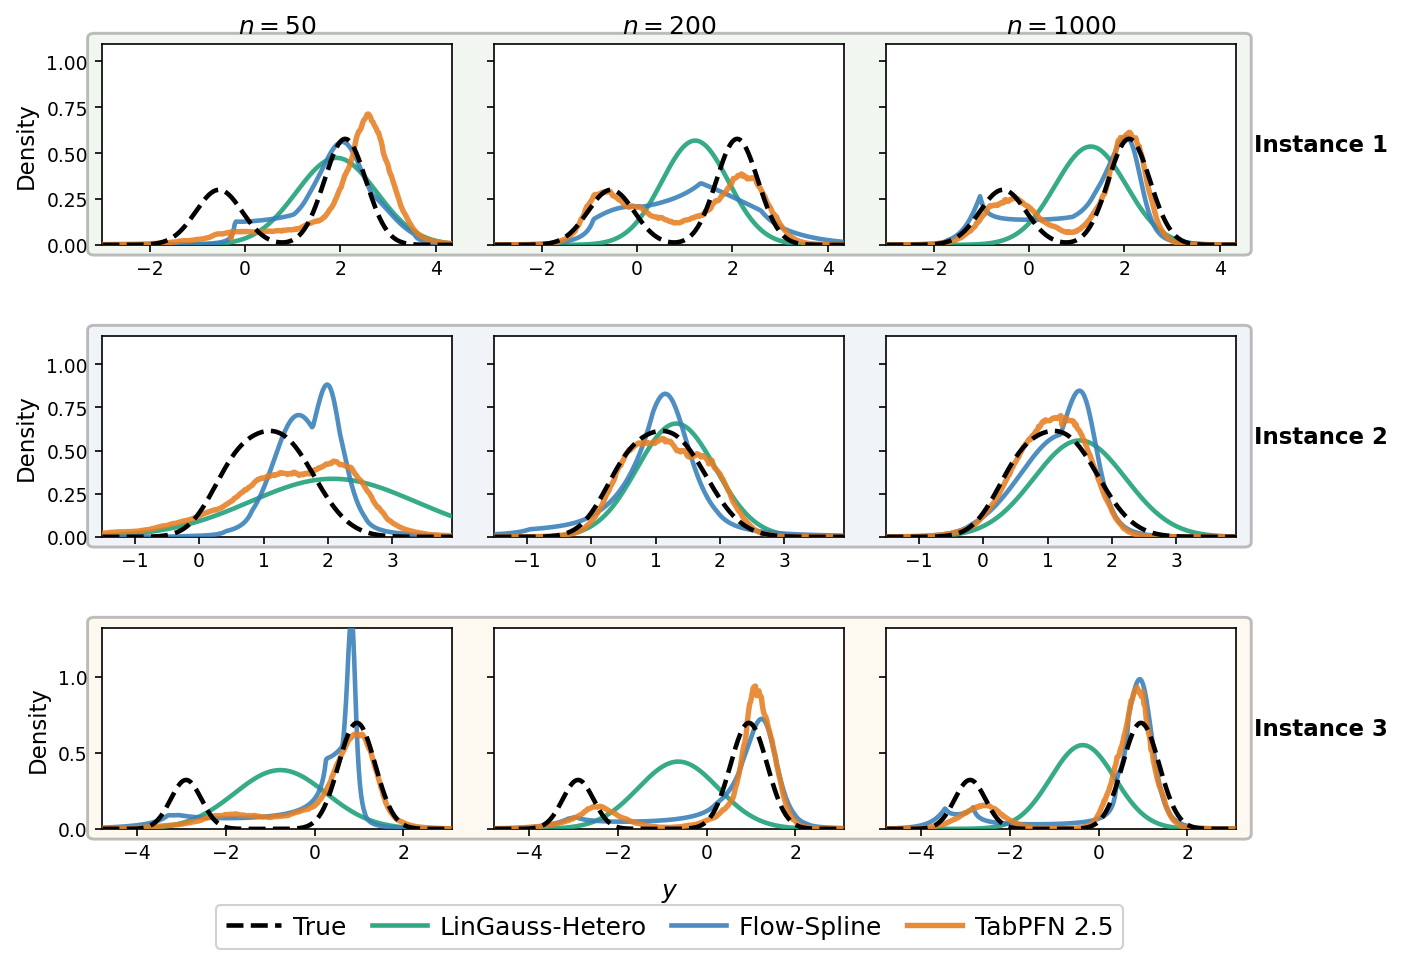
\includegraphics[scale=0.6]{results_simulated/bimodal_illustration.png}
  \caption{\textcolor{red}{\textbf{Illustration of CDE on the Bimodal synthetic DGP.}
    Each row corresponds to a different test instance with a bimodal true density (dashed black).
    Columns show three training sizes ($n\in\{50,200,1000\}$).
    \method{TabPFN~2.5} (orange) already recovers the bimodal structure at $n=50$, while
    \method{Flow-Spline} (blue) requires substantially more data to approach the truth,
    and the heteroscedastic Gaussian baseline (\method{LinGauss-Hetero}, green)
    cannot capture bimodality regardless of sample size.}}
  \label{fig:simulated}
\end{figure}

\subsection{Novelty}
\label{sec:novelty}

Our main contributions are:

\begin{itemize}[leftmargin=*]
  \item \textbf{A broad benchmark of tabular foundation models for CDE:}
    We evaluate the conditional density outputs of \method{TabPFN} and
    \method{TabICL} against a diverse set of parametric, semiparametric,
    and nonparametric baselines.

  \item \textbf{Large-scale experimental design:}
    The benchmark covers eight synthetic data-generating processes (with
    known ground-truth densities, enabling exact evaluation) and
    \textcolor{red}{thirty-nine} real-world datasets from OpenML and SDSS~DR18, with sample
    sizes ranging from \textcolor{red}{50} to 20{,}000 and covariate dimensions from
    \textcolor{red}{4} to \textcolor{red}{563}.

  \item \textbf{Multifaceted evaluation:}
    We evaluate all methods using seven complementary metrics---CDE loss,
    log-likelihood, CRPS, PIT-based calibration, 90\% coverage, interval
    width, and computation time---to assess accuracy, calibration, and
    efficiency jointly.
\end{itemize}



\section{Background}
\label{sec:background}

\subsection{Conditional Density Estimation}
\label{sec:cde_background}

Let $(X,Y)\sim P_{XY}$, where $X\in\cX\subseteq\R^d$ denotes the covariates and
$Y\in\cY\subseteq\R$ a univariate response. Conditional density estimation
(CDE) seeks to estimate the full conditional distribution of $Y$ given $X=x$.
When a conditional density exists, it is a function $f(y\mid x)$ such that
\begin{equation}
  \Prob(Y\in A\mid X=x)=\int_A f(y\mid x)\,dy
  \label{eq:cond_density}
\end{equation}
for every measurable set $A\subseteq\cY$.

Unlike mean or quantile regression, CDE aims to recover the entire shape of the
predictive distribution, including heteroscedasticity, asymmetry, heavy tails,
and multimodality. This is useful whenever downstream decisions depend on
uncertainty summaries such as predictive intervals, tail probabilities, or
quantiles. Throughout the paper, each method receives a training sample
$\cD=\{(x_i,y_i)\}_{i=1}^n$ and returns either a conditional density
$\hat f(y\mid x)$, a conditional distribution function $\hat F(y\mid x)$, or a
set of predictive quantiles from which a density can be derived.


\paragraph{Sampling from an estimated conditional distribution.}
[THINK]

\section{Methods Compared}
\label{sec:methods}

\subsection{Tabular Foundation Models}
\label{sec:methods_tfm}

We evaluate four tabular foundation model variants:
\method{TabPFN-Native}, \method{TabPFN-2.5}, \method{RealTabPFN-2.5}, and
\method{TabICL-Quantiles}
\citep{hollmann2025tabpfn,qu2025tabicl,qu2026tabiclv2}. All four models are
used as pretrained in-context learners, without task-specific gradient updates.

The three \method{TabPFN} variants output bar distributions over the response
range. \textcolor{red}{We convert these bar distributions into conditional densities as follows: for each bin, we divide the predicted probability mass by the bin width to obtain a density value at the bin center; we then interpolate these bin-center density values onto a fine evaluation grid of 200 equally spaced points using linear interpolation; finally, the interpolated density is renormalized to integrate to one. Note that this produces a linearly interpolated approximation to the underlying piecewise-constant bar density, rather than evaluating the exact step function directly.} By contrast,
\method{TabICL-Quantiles} outputs predictive quantiles. We convert these
quantiles into a conditional distribution function by interpolation and then
differentiate numerically to obtain a density. Full implementation details for
these conversions are given in Appendix~\ref{app:tfm_details}.

\subsection{Baselines}
\label{sec:methods_baselines}

To place tabular foundation models in context, we compare them with a diverse
set of classical and modern CDE baselines. These include parametric
distributional regression models
(\method{LinearGauss-Homo}, \method{LinearGauss-Hetero}, \method{Student-t},
\method{LogNormal-Homo}, \method{LogNormal-Hetero}, and \method{Gamma-GLM},
together with ridge-regularized variants), quantile-based methods
(\method{Quantile-Tree}), regression-based density
estimation via \method{FlexCode-RF} and \method{FlexZBoost} \citep{izbicki2017converting}\textcolor{red}{\citep{dalmasso2020cdetools}}, tree-based
probabilistic models (\method{BART-Homo} and \method{BART-Hetero}), and neural
density estimators (\method{MDN}, \method{Flow-Spline}, and \method{CatMLP})
\citep{bishop1994mixture,chipman2010bart,he2019xbart,durkan2019nsf,
papamakarios2021normalizing}. [fix location of citations]

These baselines span parametric, semiparametric, and nonparametric approaches,
and cover both unimodal and multimodal predictive families. Their role in the
benchmark is not to identify a single best CDE strategy in general, but to
provide strong and diverse comparison points for assessing the density quality,
calibration, and computational profile of tabular foundation models. Detailed
implementation choices for each baseline are reported in
Appendix~\ref{app:baseline_details}.

% ===================================================================
%  4. EXPERIMENTAL SETUP
% ===================================================================
\section{Experimental Setup}
\label{sec:setup}

We evaluate four tabular foundation model variants and a diverse set of
parametric, tree-based, and neural baselines on synthetic and real-world
regression tasks. Experiments vary the dataset and training-set size, and all
methods are assessed using proper scoring rules, calibration diagnostics,
interval-based summaries, and computation time. Unless otherwise noted, results
are averaged over \textcolor{red}{4} independent repetitions.

\subsection{Evaluation Metrics}
\label{sec:metrics}

We evaluate all methods using seven complementary metrics covering density
accuracy, calibration, sharpness, and computational cost. Let $\hat f(y\mid x)$
denote an estimated conditional density and let
\begin{equation}
  \hat F(y\mid x)=\int_{-\infty}^{y}\hat f(t\mid x)\,dt
  \label{eq:estimated_cdf}
\end{equation}
be the associated predictive distribution function. When a method outputs
$\hat F$ or predictive quantiles directly, we evaluate the corresponding implied
distribution.

Our main density-specific metric is the CDE loss
\citep{izbicki2017converting},
\begin{equation}
  L(\hat f)=\int\!\!\int \hat f(y\mid x)^2\,dy\,dP_X(x)
  -2\,\E_{(X,Y)}[\hat f(Y\mid X)].
  \label{eq:cde_loss}
\end{equation}
This is a proper scoring rule, minimized in expectation by the true conditional
density. For synthetic datasets, where the data-generating process is known, we
evaluate this loss using the known conditional distribution rather than a purely
empirical surrogate \textcolor{red}{(the first integral is computed analytically and the second is estimated on the held-out test set)}. For real-world datasets, we estimate it on held-out test
data.


A CDE is calibrated if events predicted to occur with a given probability occur with approximately that same frequency under the data-generating distribution. In the conditional-distribution setting, a standard notion of probabilistic calibration is that, when $(X,Y)$ is drawn from the test distribution, the random variable $
U = \hat F(Y \mid X)$
should be approximately uniformly distributed on $[0,1]$. Departures from uniformity indicate that the predictive distribution is systematically too narrow, too wide, or otherwise misspecified.  [MERGE BETTER; ADD REFS]

We also report mean test log-likelihood and the continuous ranked probability
score (CRPS) \citep{gneiting2007strictly} as proper scoring rules; the
Kolmogorov--Smirnov statistic of the probability integral transform (PIT) values
as a calibration diagnostic \citep{zhao2021diagnostics}; empirical coverage  of 90\% predictive intervals; and total fit-and-predict wall-clock
time. Together, these metrics distinguish methods that are accurate as density
estimators, well calibrated as probabilistic predictors, and practical in terms
of computation.

\subsection{Protocol and Hyperparameter Tuning}
\label{sec:protocol}

Each experiment is repeated over \textcolor{red}{4} independent train/test splits. \textcolor{red}{In each split, 25\% of the available data is held out as the test set.} We report the
mean of each metric across repetitions together with standard errors. \textcolor{red}{Complete numerical results, including standard errors for all methods and datasets, are available at \url{https://github.com/rizbicki/tabDensityComparisons}.}
All
tabular foundation models are used with their default pretrained settings.

For the baselines, hyperparameters are selected on the training data only.
Ridge-regularized parametric models choose the regularization strength by
cross-validation; \method{FlexCode-RF} selects the number of basis functions by
cross-validation; and the remaining baselines are tuned by random search with
cross-validation using the CDE loss as the selection criterion. After tuning,
the selected configuration is refit on the full training set. Complete search
spaces and implementation details are reported in
Appendix~\ref{app:tuning_details}.

\subsection{Datasets}
\label{sec:datasets}

We include \textcolor{red}{39} regression datasets from OpenML and SDSS~DR18
\citep{sdss_dr18}, spanning domains such as housing, robotics, computer
hardware, transportation, molecular prediction, retail, \textcolor{red}{music, bioinformatics, energy,} and photometric
redshift estimation. \textcolor{red}{The covariate dimension $d$ (after one-hot encoding of categorical features) ranges from 5 to 563 across the real-world datasets.}
For each dataset, we evaluate methods on nested subsamples
of size $n \in \{$\textcolor{red}{50, 500,} $1{,}000$\textcolor{red}{, 5{,}000, 10{,}000,} $20{,}000\}$ whenever
available. Complete dataset details are reported in
Appendix~\ref{app:real_datasets}.


\section{Results}
\label{sec:results}

\textcolor{red}{Figures~\ref{fig:rankings_cde_n50}--\ref{fig:rankings_cde_n20000} present CDE loss raw-value heatmaps across real-world datasets at $n \in \{50, 1{,}000, 20{,}000\}$, with datasets sorted by covariate dimension $d$.
At every sample size, the four tabular foundation model variants (orange) occupy the top four positions in average rank.}

\textcolor{red}{At $n=50$ (Figure~\ref{fig:rankings_cde_n50}), \method{TabPFN-2.5} achieves an average rank of 2.6 across the 39 datasets, with \method{RealTabPFN-2.5} (2.9) and \method{TabPFN-Native} (3.4) close behind, and \method{TabICL-Quantiles} (8.3) also ahead of all non-foundation baselines.
Among the latter, the best performers are \method{Student-t-Ridge} (7.8) and \method{FlexCode-RF} (9.0).}

\textcolor{red}{At $n=1{,}000$ (Figure~\ref{fig:rankings_cde_n1000}), the four foundation models maintain the top four average ranks: \method{TabPFN-Native} and \method{RealTabPFN-2.5} are tied at 2.5, \method{TabPFN-2.5} is at 2.9, and \method{TabICL-Quantiles} is at 3.2.
Among non-foundation baselines, \method{FlexCode-RF} (9.2) and \method{Quantile-Tree} (9.2) perform best. Parametric baselines and BART variants consistently rank in the lower half regardless of regularization.}

\textcolor{red}{At $n=20{,}000$ (Figure~\ref{fig:rankings_cde_n20000}, which covers only the 16 datasets large enough for this subsample), \method{TabPFN-2.5} remains first (2.7), with \method{TabPFN-Native} (3.4), \method{RealTabPFN-2.5} (3.0), and \method{TabICL-Quantiles} (4.0) also in the top four.
The gap between foundation models and flexible nonparametric baselines such as \method{Flow-Spline} (5.0) and \method{MDN} (6.6) narrows as $n$ grows, consistent with a sample efficiency advantage of foundation models at small $n$.}

\begin{figure}[H]
  \centering
  
\includegraphics[scale=0.6]{results_real/raw_real_cde_loss_n50}
  \caption{\textbf{CDE loss across real-world datasets at
    $n = 50$.}
    Per-dataset raw CDE loss values (lower/greener is better).
    The datasets are sorted by covariate dimension $d$.
    \textcolor{red}{All four tabular foundation models (orange, rightmost columns) rank in the top four by average rank (bottom row), with \method{TabPFN~2.5} achieving the best average rank of 2.6. Even at this extremely small sample size, foundation models outperform all parametric and nonparametric baselines.}
    Results at other sample sizes are reported in
    Appendix~\ref{app:rankings}.}
  \label{fig:rankings_cde_n50}
\end{figure}

\begin{figure}[H]
  \centering
  
\includegraphics[scale=0.6]{results_real/raw_real_cde_loss_n1000}
  \caption{\textbf{CDE loss across real-world datasets at
    $n = 1{,}000$.}
    Per-dataset raw CDE loss values (lower/greener is better).
    The datasets are sorted by covariate dimension $d$.
    \textcolor{red}{Foundation models (orange) occupy the top four average ranks; \method{TabPFN-Native} and \method{RealTabPFN-2.5} tie at rank 2.5. Among non-foundation methods, \method{FlexCode-RF} and \method{Quantile-Tree} are the strongest competitors (average rank $\approx$9.2), but remain well behind the foundation models.}
    Rankings at other sample sizes are reported in
    Appendix~\ref{app:rankings}.}
  \label{fig:rankings_cde_n1000}
\end{figure}

\begin{figure}[H]
  \centering
  
\includegraphics[scale=0.5]{results_real/raw_real_cde_loss_n20000}
  \caption{\textbf{CDE loss across real-world datasets at
    $n = 20{,}000$.}
    Per-dataset raw CDE loss values (lower/greener is better; only the \textcolor{red}{16} datasets with at least 20{,}000 observations are included).
    The datasets are sorted by covariate dimension $d$.
    \textcolor{red}{Foundation models still dominate: \method{TabPFN-2.5} ranks first (avg.\ rank 2.7) and the gap with flexible nonparametric baselines (\method{Flow-Spline}: 5.0, \method{MDN}: 6.6) has narrowed compared to smaller $n$, suggesting that flexible baselines benefit more from additional data.}
    Rankings at other sample sizes are reported in
    Appendix~\ref{app:rankings}.}
  \label{fig:rankings_cde_n20000}
\end{figure}



\begin{figure}[H]
  \centering
  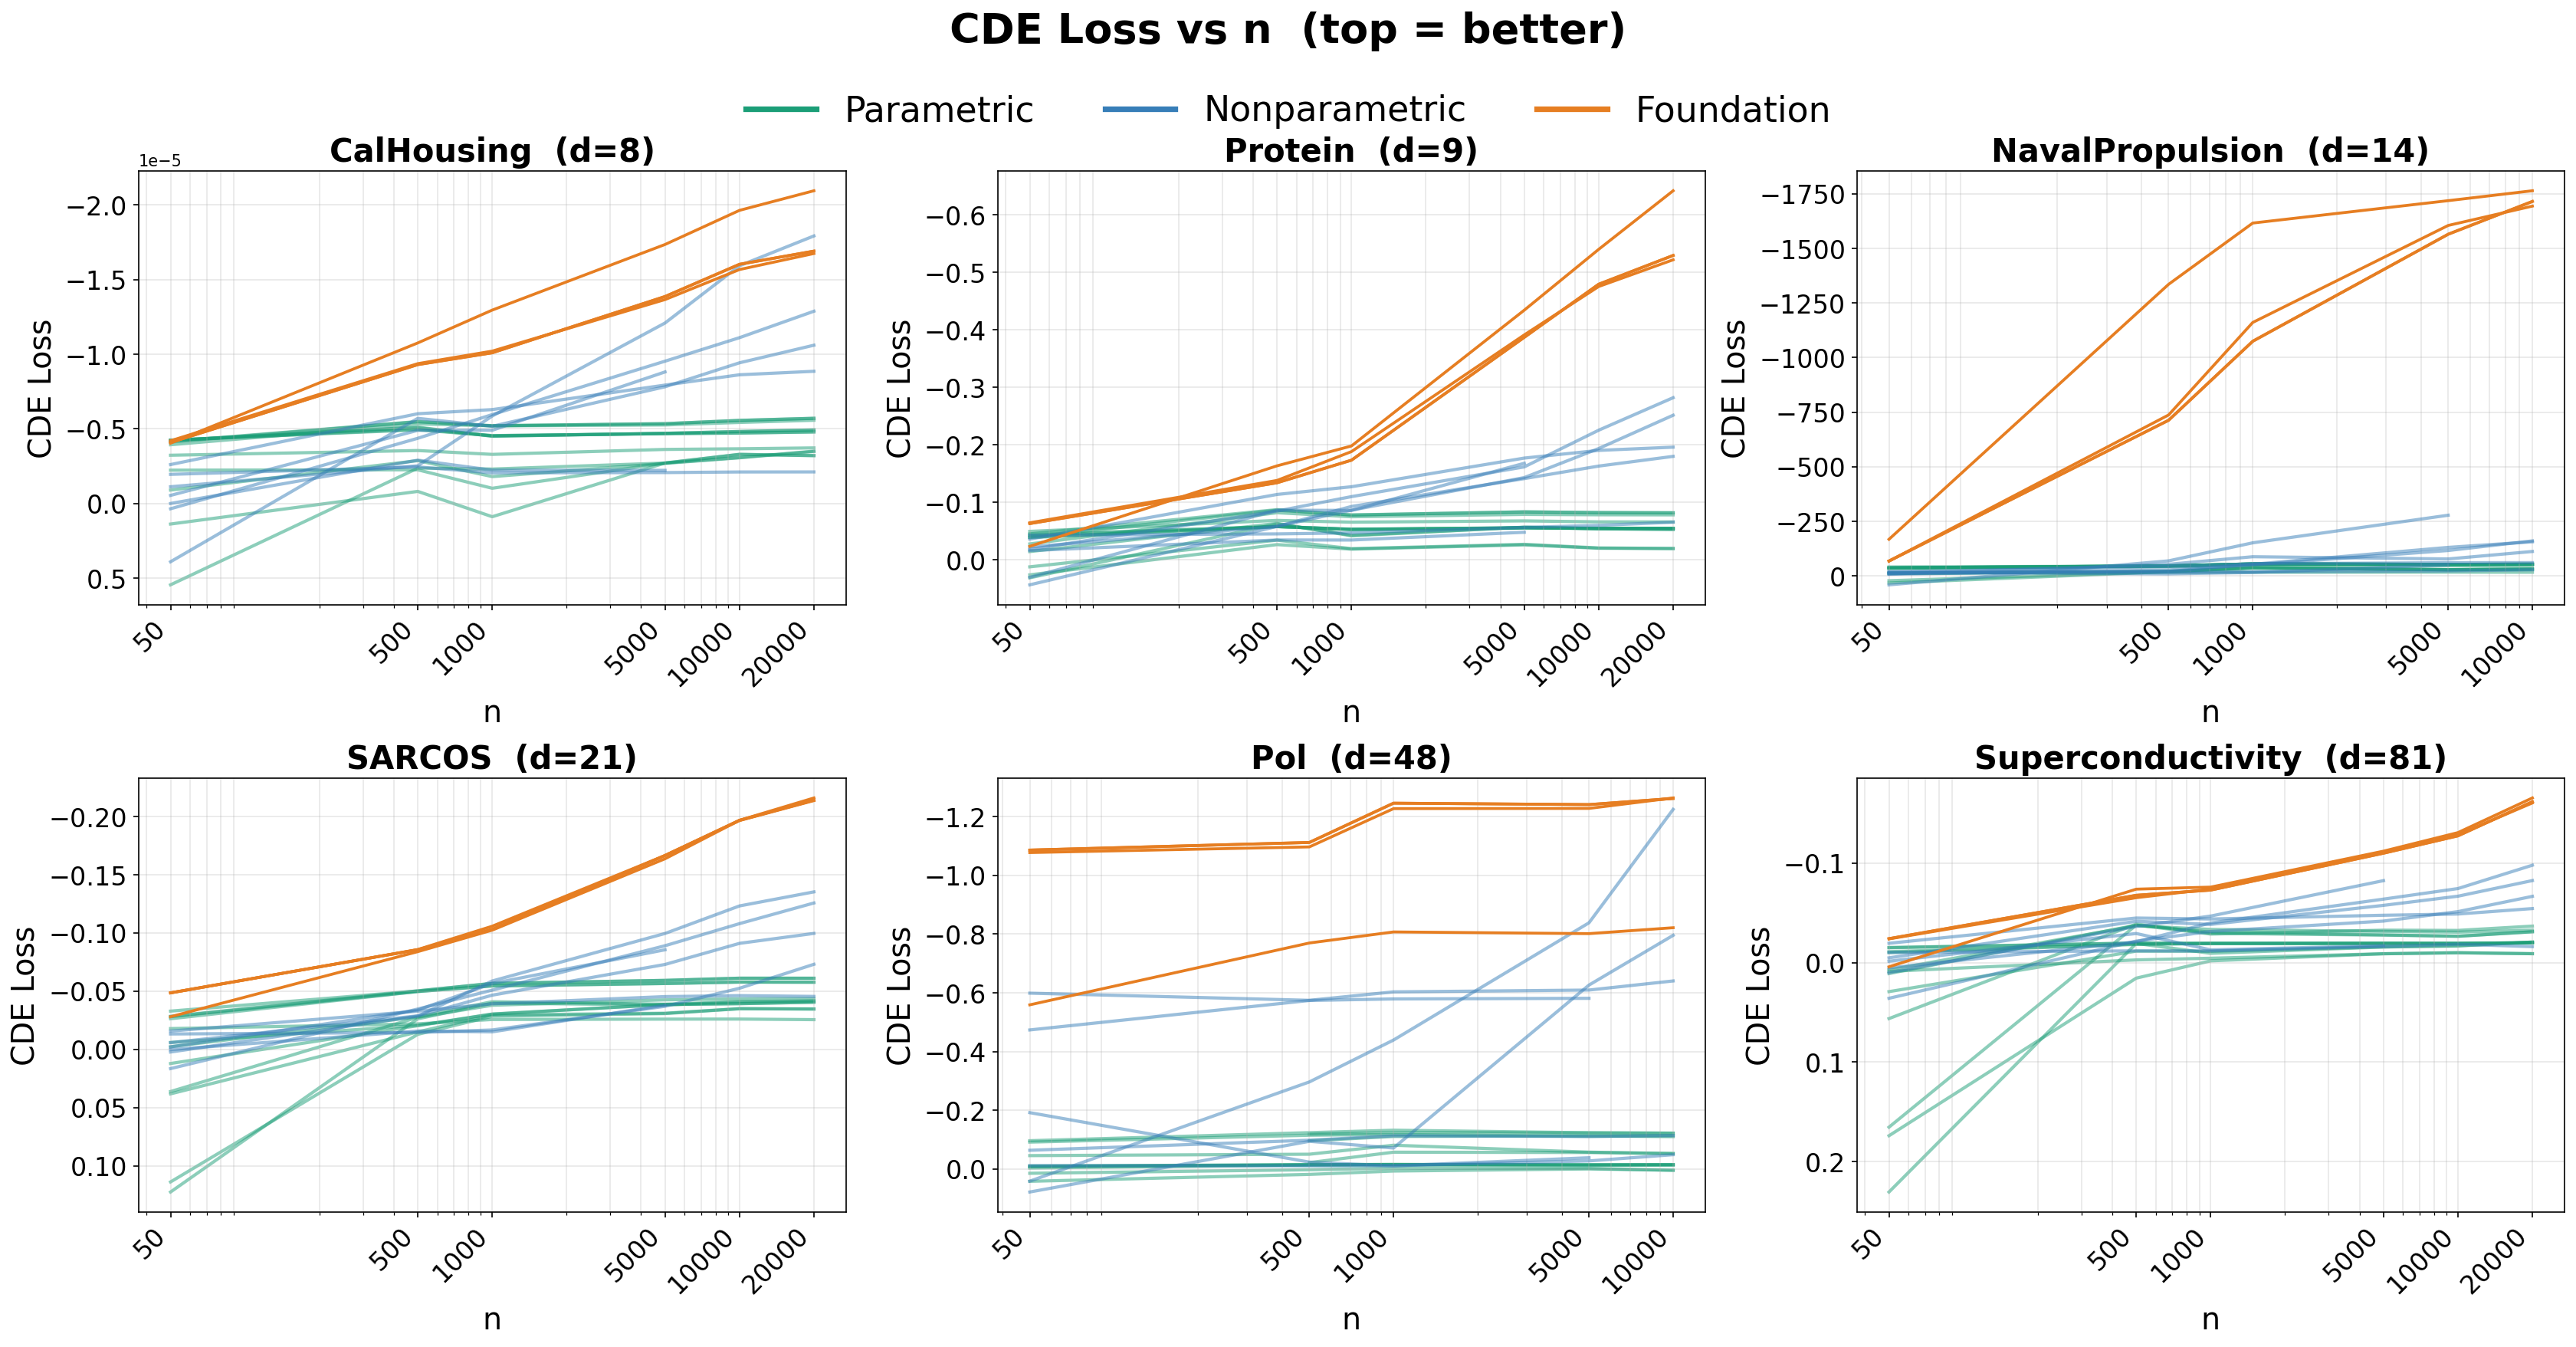
\includegraphics[width=\linewidth]{results_real/perf_vs_n_foundational_cde_loss_real_by_d.png}
  \caption{\textbf{CDE loss vs.\ sample size on real-world datasets,
    highlighting foundation models.}
    \textcolor{red}{Each panel shows one real-world dataset; foundation models (orange) are compared against parametric (green) and nonparametric (blue) baselines.
    Foundation models are most dominant at small~$n$ and the advantage persists as $n$ grows, though flexible nonparametric baselines tend to close the gap on larger datasets. Datasets are arranged by increasing covariate dimension.}
    Analogous plots for synthetic datasets and other metrics are in
    Appendix~\ref{app:perf_vs_n}.}
  \label{fig:perf_vs_n_real}
\end{figure}


[comment something about performance according to log-lik and CRPS, but only mention appendix]

[comment something about calibration based on plots in appendix; but only refer to appendix]

\subsection{Results on Synthetic Data}
\label{sec:results_synthetic}

The synthetic benchmarks, where the true conditional density is known
in closed form, allow us to assess performance without the confounding
effects of model misspecification relative to an unknown ground truth.
[To expand: summarize rankings on synthetic data, discuss how
foundation models perform on bimodal, skewed, and heteroscedastic
DGPs.
Reference synthetic ranking heatmaps and performance-vs-$n$ curves
in the appendix.]



\section{Case Study: Photometric Redshift Estimation with SDSS}
\label{sec:sdss}

The benchmark results in Section~\ref{sec:results} compare all methods at
sample sizes up to $n = 20{,}000$, which falls within the context-length
budget of current tabular foundation models.
A natural question is how these models fare on a genuinely large-scale
scientific dataset, and---more importantly---how their performance at
moderate~$n$ compares to classical methods that can leverage much larger
training sets.
To investigate this, we conduct a dedicated scaling study on photometric
redshift estimation using the Sloan Digital Sky Survey (SDSS) Data
Release~18 \citep{sdss_dr18}.


[maybe say that the field has dedicated groups to estimate such density]
The SDSS dataset consists of approximately 500{,}000 galaxies with
$ugriz$ broadband photometric magnitudes as features ($d=5$) and spectroscopic
redshift as the response.
Estimating the full conditional density $f(z \mid \text{photometry})$
is a canonical CDE task in astrophysics: downstream cosmological
analyses require well-calibrated photo-$z$ distributions rather than
mere point estimates \citep{schmidt2020evaluation,izbicki2017photo}.
We subsample the full dataset at
$n \in \{$\textcolor{red}{500,\, 1{,}000,}$\, 10\text{k},\, 50\text{k},\, 100\text{k},\, 250\text{k},\, 500\text{k}\}$
using nested deterministic subsamples (so that each smaller set is a
strict subset of the next larger one), and run each method--size
combination over \textcolor{red}{5} repetitions with independent train/test splits.
Tabular foundation models are subject to context-length constraints:
\method{TabPFN} variants are evaluated up to $n = 50{,}000$ \textcolor{red}{on GPU} and
\method{TabICL-Quantiles} up to \textcolor{red}{$n = 100{,}000$} (on GPU), beyond which
they \textcolor{red}{are not evaluated in this study}.
All other methods are evaluated at all sample sizes up to \textcolor{red}{500k} where
computationally feasible.

\textcolor{red}{In addition to the methods in the main benchmark, we also evaluate \method{FlexZBoost}, a sharpening-enhanced variant of \method{FlexCode} with XGBoost regressors \citep{dalmasso2020cdetools}, which has shown strong performance for photometric redshift estimation tasks \citep{schmidt2020evaluation}.}


Figure~\ref{fig:sdss_scaling} presents CDE loss as a function of
training set size for all method families.
The most striking finding is the sample efficiency of the foundation
models.
At $n = 50{,}000$---the largest training set they can process---the
\method{TabPFN} variants achieve a CDE loss of approximately $-11$,
which is substantially lower (better) than every parametric and
GLM-based baseline evaluated at $n = 500{,}000$, the full dataset.
In other words, the tabular foundation models, when conditioned on only 10\% of the target dataset at inference time, outperform standard approaches that have access to the entire sample.

Among the nonparametric baselines, \method{Flow-Spline} is the
only method that eventually reaches a comparable CDE loss, but it
requires roughly $n = 250{,}000$ training samples to approach the
performance that the foundation models achieve at $n = 50{,}000$---a
five-fold difference in data requirements.
\method{MDN} also improves steadily with~$n$ but plateaus at a
CDE loss around $-8.5$ to $-9$ even at the largest sample sizes,
remaining well below the foundation model curve.
The parametric baselines (best represented by \method{Student-t} in the figure),
show comparatively little improvement beyond $n = 50{,}000$ and
cluster around the $-4$ to $-5$ CDE loss range, reflecting the
fundamental limitation of misspecified distributional assumptions for
this dataset.

These results highlight a practical advantage of tabular foundation
models: in settings where data acquisition is expensive or where
computational resources limit the training set size that downstream
methods can handle, the distributional outputs of \method{TabPFN}
provide CDE quality that would otherwise require an order of magnitude
more data with conventional approaches.

[full results in Appendix XXXX]

[comment on log scale]


\begin{figure}[hp!]
  \centering
  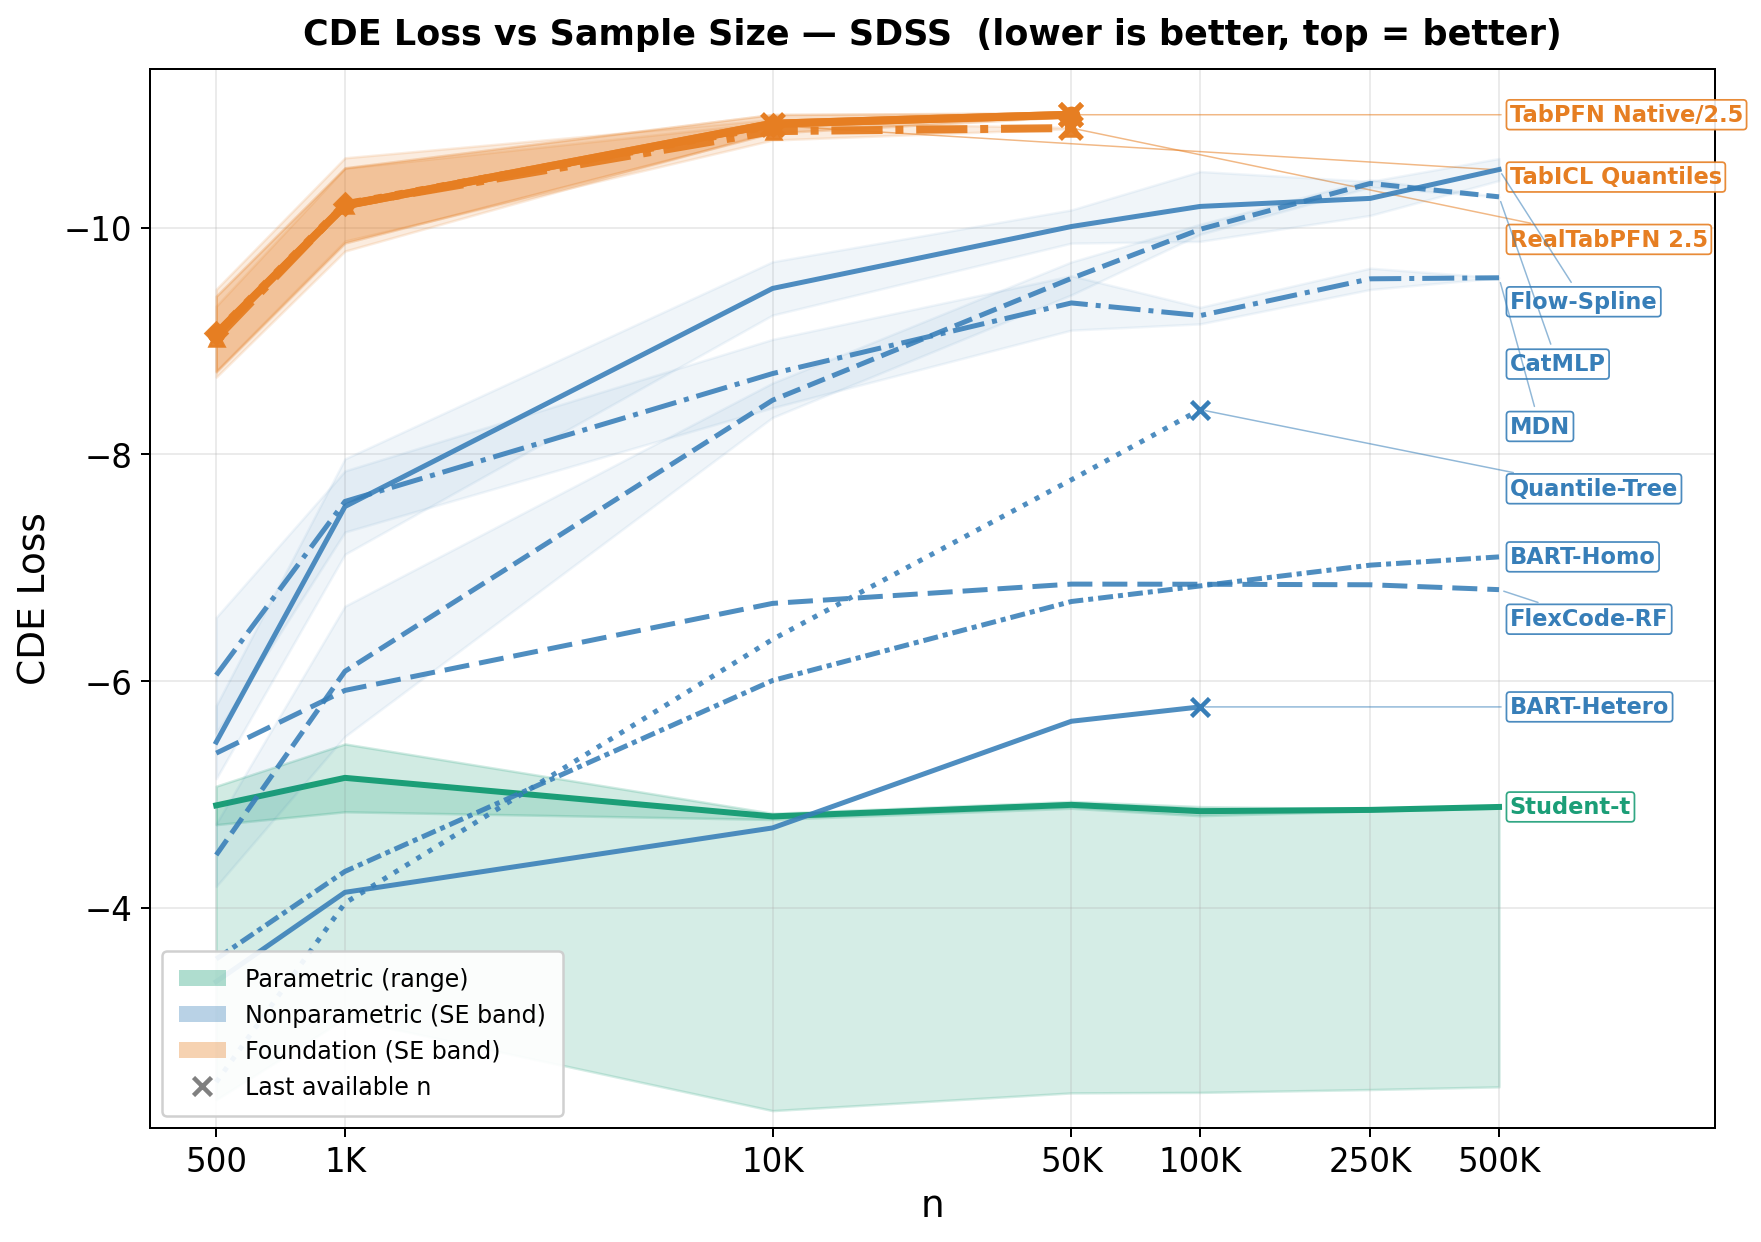
\includegraphics[scale=0.55]{sdss/perf_vs_n_cde_loss_improved.png}
  \caption{\textcolor{red}{\textbf{CDE loss vs.\ training sample size on the SDSS photometric redshift dataset}} (lower is better; $y$-axis inverted so top = better).
\textbf{Parametric methods} (green): the shaded band spans the full
range across all parametric models; the best-performing parametric model (\method{Student-t}) is highlighted as a solid line.
Ridge-regularized variants are omitted from the band as they are
uniformly worse and would distort the $y$-axis scale.
\textbf{Nonparametric methods} (blue): each method is shown as a
separate line; shaded $\pm1$ SE bands are displayed only for the
best-performing nonparametric methods to avoid visual clutter.
A terminal $\times$ marker indicates the last sample size at which a
method was evaluated.
\textbf{Foundation models} (orange): \method{TabPFN-Native} and \method{TabPFN~2.5} produce near-identical results and are shown as a single merged label (\method{TabPFN Native/2.5});
\method{RealTabPFN-2.5} and \method{TabICL-Quantiles} are shown separately.
\textcolor{red}{\textbf{Key finding:} \method{TabPFN} trained on 50k galaxies outperforms all parametric methods trained on 500k galaxies, demonstrating a ten-fold data efficiency advantage.}
SE estimates are computed across 5 independent train/test splits.}
  \label{fig:sdss_scaling}
\end{figure}


\begin{figure}[H]
  \centering
  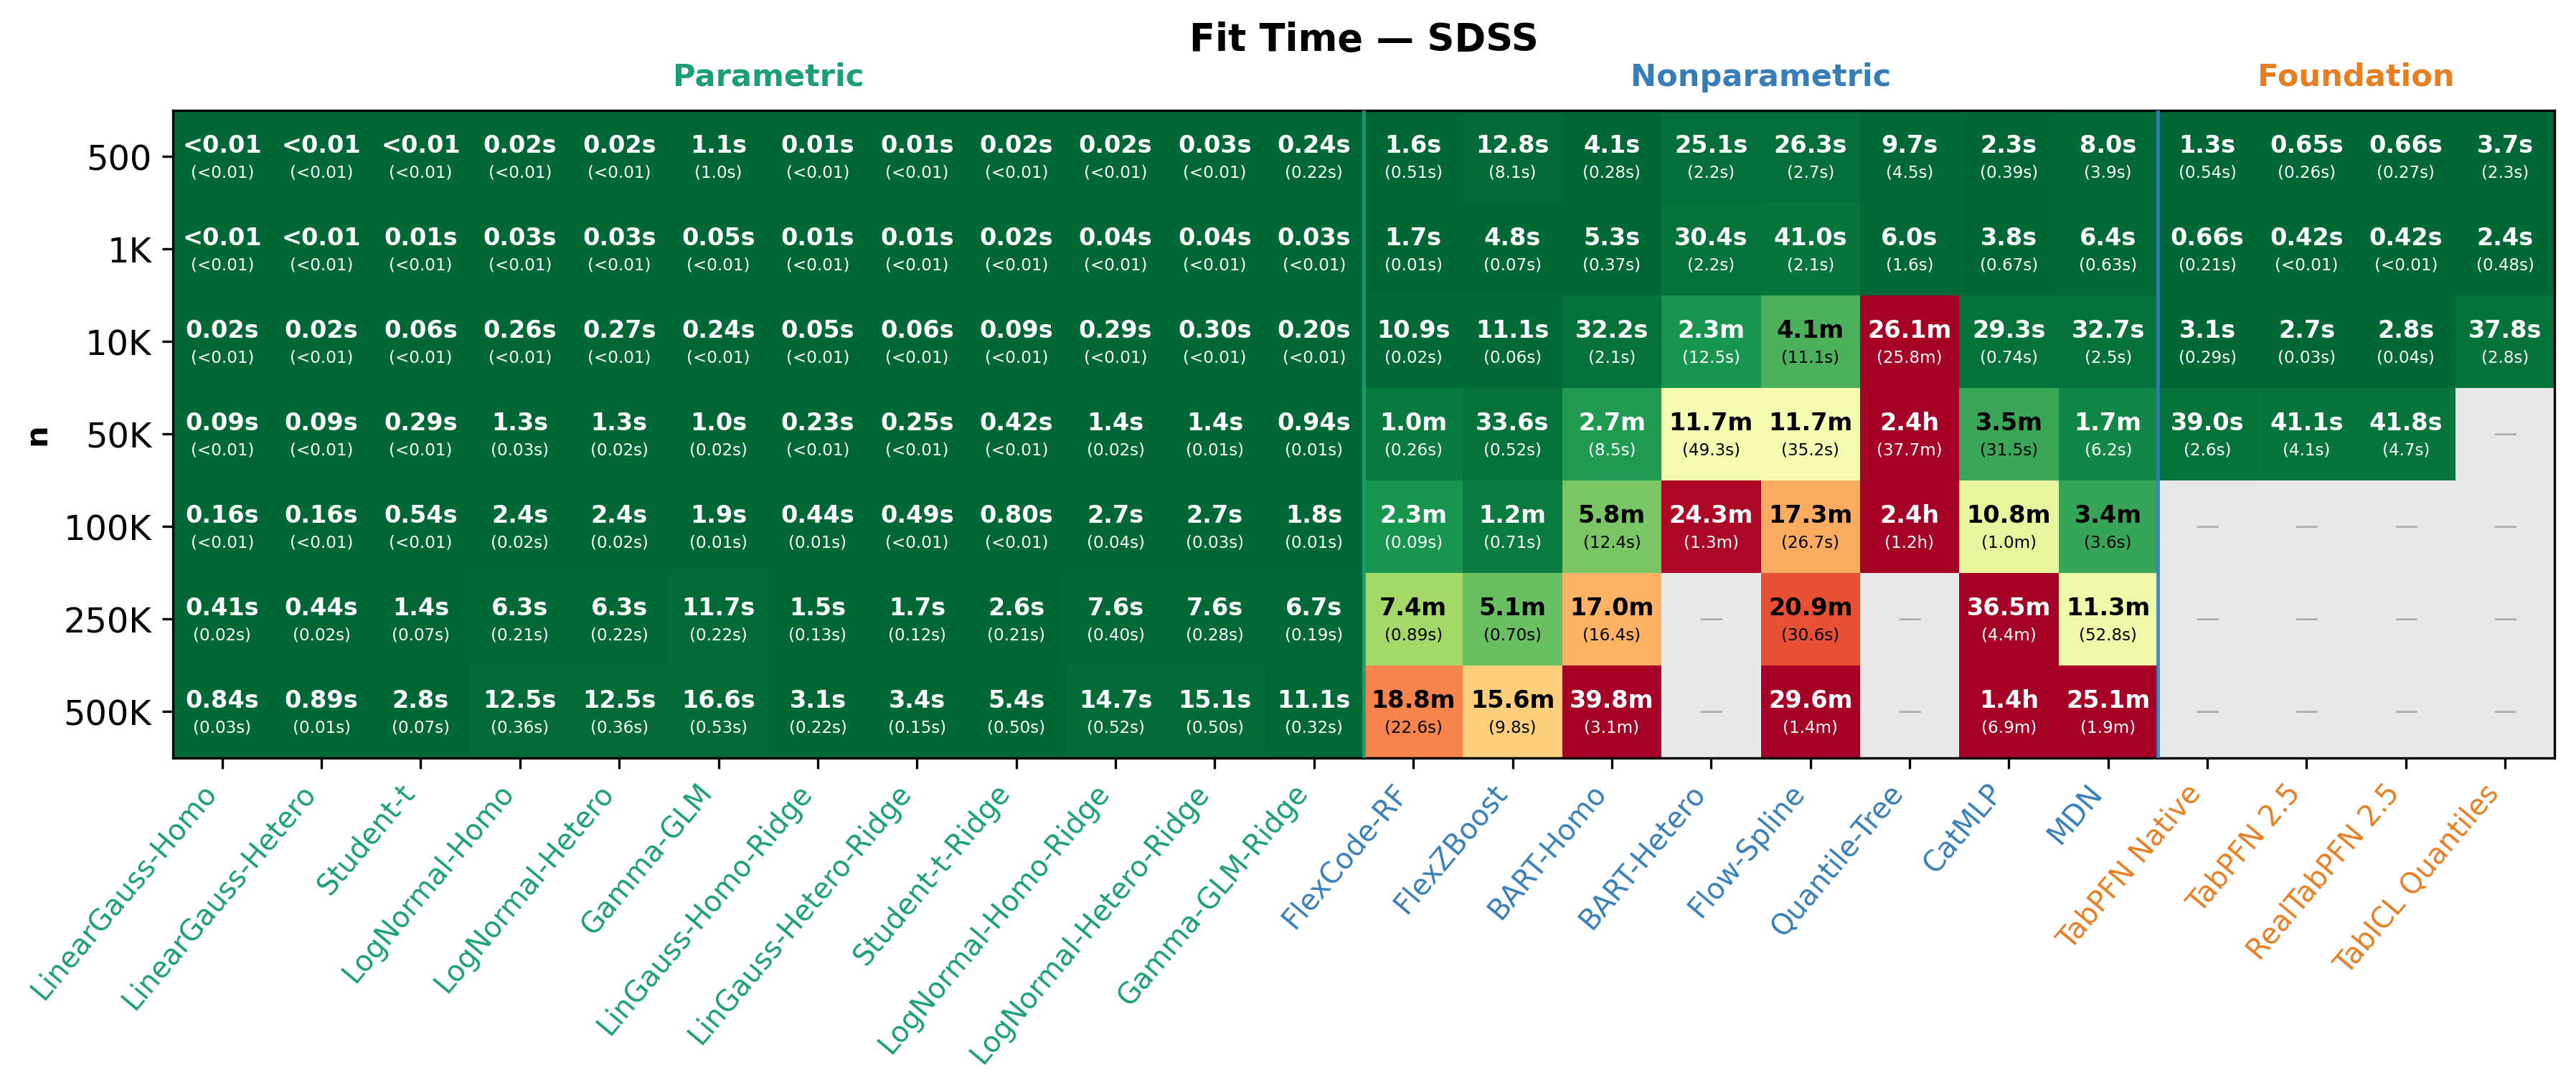
\includegraphics[width=\linewidth]{sdss/raw_real_fit_time_sdss.png}
  \caption{\textcolor{red}{\textbf{Fit time (training + prediction) for each method across sample sizes~$n$ on the SDSS photometric redshift dataset.}}
Each cell reports the mean fit time (top) and standard error in
parentheses.
Cells are colour-coded within each method column from green (fastest)
to red (slowest); grey cells indicate that the method was not run
at that sample size due to computational limits.
Fit time includes both training and inference on the test set.
\textcolor{red}{\textbf{Key finding:} Foundation models are substantially faster than neural baselines (\method{Flow-Spline}, \method{MDN}) at the same sample sizes, while parametric baselines are the cheapest overall but sacrifice density accuracy.}
}
  \label{fig:sdss_fit_time}
\end{figure}


\section{Final Remarks}
\label{sec:final}

[mention we didn't even do fine tuning and used models combined models with larger n's]

[extend to multivariate response?]

[calibracao]

Code to reproduce all experiments and regenerate all figures is available
at \url{https://github.com/rizbicki/tabDensityComparisons}. \textcolor{red}{The repository also provides a full HTML summary of all experimental results, including per-dataset metric values and standard errors across all methods, sample sizes, and evaluation metrics.}


% ===================================================================
%  ACKNOWLEDGEMENTS
% ===================================================================
\section*{Acknowledgements}



% ===================================================================
%  REFERENCES
% ===================================================================
\bibliography{references}
\bibliographystyle{tmlr}


% ===================================================================
%  APPENDIX
% ===================================================================
\appendix



\section{Implementation Details}
\label{app:implementation}

\subsection{From Foundation-Model Outputs to Densities}
\label{app:tfm_details}

\paragraph{\method{TabPFN-Native}.}
\method{TabPFN} is a transformer trained through in-context learning on
synthetic tabular tasks sampled from a prior over data-generating mechanisms
\citep{hollmann2025tabpfn}. In regression mode, it outputs a bar distribution:
a discrete probability mass over bins that partition the response range. \textcolor{red}{We convert this bar distribution to a conditional density as follows: for each bin, the probability mass is divided by the bin width to obtain a density value at the bin center; these bin-center density values are then linearly interpolated onto a fine evaluation grid of 200 equally spaced points spanning the training range (plus a 5\% margin on each side); finally, the interpolated density is clamped to be non-negative and renormalized to integrate to one. This procedure yields a smooth approximation to the underlying piecewise-constant bar density rather than evaluating the exact step function.}

\paragraph{\method{TabPFN-2.5}.}
This variant uses the explicit v2.5 default regression checkpoint from the
\method{TabPFN} release \citep{hollmann2025tabpfn}. \textcolor{red}{The density extraction
procedure is identical to \method{TabPFN-Native}: bar-distribution outputs are
accessed via \texttt{output\_type="full"}, bin probabilities are divided by bin
widths to obtain bin-center density values, which are then linearly interpolated
onto the 200-point evaluation grid and renormalized.}

\paragraph{\method{RealTabPFN-2.5}.}
This variant uses the \method{RealTabPFN} regression checkpoint from the
\method{TabPFN~v2.5} release \citep{hollmann2025tabpfn}. The prediction
interface is the same as for \method{TabPFN-2.5}, but the model is additionally
fine-tuned on curated real-world tabular datasets. As with the other
\method{TabPFN} variants, we use its native bar distribution as the starting
point for the CDE output, \textcolor{red}{following the same interpolation procedure described above}.

\paragraph{\method{TabICLv2-Quantiles}.}
\method{TabICL} also follows an in-context learning paradigm for tabular
prediction, but uses a different architecture and pretraining strategy
\citep{qu2025tabicl,qu2026tabiclv2}. \textcolor{red}{We use an ensemble of four estimators (\texttt{n\_estimators=4}).} Its
regression variant outputs predictive quantiles. We extract 199 quantiles at
levels $\alpha \in \{0.005, 0.010, \ldots, 0.995\}$, enforce monotonicity by
sorting, and interpolate the resulting quantile function onto a regular grid to
obtain the CDF. The conditional density is then computed as the numerical
gradient of the interpolated CDF, clamped to be non-negative and renormalized.

\subsection{Baseline Implementations}
\label{app:baseline_details}

\subsubsection{Parametric baselines}
\label{app:parametric_details}

These methods assume a parametric family for $Y\mid X=x$ and allow one or more
distributional parameters to depend on the covariates.

\paragraph{\method{LinearGauss-Homo}.}
A Gaussian linear model with mean linear in $x$ and constant variance:
$Y\mid X=x\sim\mathcal N(\beta^\top x,\sigma^2)$, where $\hat\sigma^2$ is
estimated from training residuals with a degrees-of-freedom correction
\citep{rigby2005generalized,kneib2023rage}.

\paragraph{\method{LinearGauss-Hetero}.}
A heteroscedastic Gaussian model in which both the mean and the variance depend
on $x$ \citep{rigby2005generalized,kneib2023rage}. In the first stage, the
conditional mean is fit by ordinary linear regression,
$\hat\mu(x)=x^\top\hat\beta$. In the second stage, the log-squared residuals are
regressed on $x$:
$\log(\hat\varepsilon^2)=x^\top\hat\gamma$, yielding a covariate-dependent
standard deviation
$\hat\sigma(x)=\sqrt{\exp(x^\top\hat\gamma)}$. The predictive density is then
$\hat f(y\mid x)=\mathcal N(y;\hat\mu(x),\hat\sigma(x)^2)$.

\paragraph{\method{Student-t}.}
A linear model with Student-$t$ conditional distribution
\citep{rigby2005generalized,kneib2023rage,klein2024distributional}. The
conditional mean is estimated by linear regression,
$\hat\mu(x)=x^\top\hat\beta$. The degrees of freedom $\hat\nu$ and scale
$\hat\sigma$ are then estimated by profile maximum likelihood on the training
residuals, optimizing $\nu$ over $[2.01,200]$ and setting
$\hat\sigma=\sqrt{\overline{\varepsilon^2}(\hat\nu-2)/\hat\nu}$ when
$\hat\nu>2$.

\paragraph{\method{LogNormal-Homo} and \method{LogNormal-Hetero}.}
These models assume a log-normal conditional distribution with linear structure
in the log-scale mean \citep{rigby2005generalized,kneib2023rage}. When the
response is not strictly positive, all training values are shifted by a
constant
$c=-\min(y_{\text{train}})+0.01\cdot\mathrm{range}(y_{\text{train}})$
so that the shifted response $\tilde Y=Y+c>0$. The model is then
$\log \tilde Y\mid X=x \sim \mathcal N(x^\top\beta,\sigma^2)$, with either
constant $\sigma$ (\method{-Homo}) or input-dependent $\sigma(x)$ estimated via
a second-stage regression on log-squared residuals (\method{-Hetero}),
analogously to \method{LinearGauss-Hetero}. The density is evaluated on the
original scale and renormalized.

\paragraph{\method{Gamma-GLM}.}
A gamma generalized linear model with a log link for the conditional mean
\citep{rigby2005generalized,kneib2023rage,klein2024distributional}. As with
the log-normal models, when the response is not strictly positive the training
values are shifted by
$c=-\min(y_{\text{train}})+0.01\cdot\mathrm{range}(y_{\text{train}})$. On the
shifted data, $\log \hat\mu(x)=x^\top\hat\beta$ is estimated by regressing
$\log\tilde y$ on $x$, and a constant shape parameter $\hat a$ is estimated
from the variance of the log-scale residuals as
$\hat a=1/\mathrm{Var}(\log\tilde y-x^\top\hat\beta)$. The predictive density
is
$\hat f(\tilde y\mid x)=\mathrm{Gamma}(\tilde y;\,a=\hat a,\,
\mathrm{scale}=\hat\mu(x)/\hat a)$, evaluated on the original scale and
renormalized.

For each parametric model above, we also include a ridge-regularized variant
(\method{-Ridge} suffix), where the regression coefficients are estimated by
ridge regression with the regularization strength selected by leave-one-out
cross-validation over 20 log-spaced values in $[10^{-4},10^4]$.

\subsubsection{Nonparametric and flexible baselines}
\label{app:nonparametric_details}

\paragraph{\method{FlexCode-RF}.}
\method{FlexCode} represents the conditional density through a cosine
orthonormal basis expansion on the normalized response:
$\hat f(z\mid x)=\sum_{i=0}^{I-1}\hat\beta_i(x)\varphi_i(z)$, where
$\varphi_0\equiv 1$ and
$\varphi_i(z)=\sqrt{2}\cos(i\pi z)$ for $i\geq 1$
\citep{izbicki2017converting}. Each coefficient function $\hat\beta_i(x)$ is
estimated by regressing $\varphi_i(Y)$ on $X$ using a random forest with 100
trees and maximum depth 8. The number of basis functions is selected by
cross-validation, and the estimated density is projected to be non-negative and
renormalized.

\paragraph{\textcolor{red}{\method{FlexZBoost}.}}
\textcolor{red}{\method{FlexZBoost} is a variant of \method{FlexCode} that replaces the random forest regression engine with XGBoost (100 trees, maximum depth 4, learning rate 0.1) and adds a post-hoc sharpening step \citep{dalmasso2020cdetools}. After fitting the basis expansion, the estimated density is raised to a power $\alpha > 0$ and renormalized; the sharpening parameter $\alpha$ is tuned by 5-fold cross-validation minimizing the CDE loss, over a grid of 16 values in $[0.5,\, 2.0]$. This method has been shown to perform well on photometric redshift estimation tasks \citep{schmidt2020evaluation}.}

\paragraph{\method{BART-Homo}.}
This method uses XBART to model the conditional mean and pairs it with a
constant residual variance estimated from the posterior mean of the XBART
$\sigma$ draws, averaged over post-burn-in sweeps, inducing a Gaussian
predictive density \citep{chipman2010bart,he2019xbart}.

\paragraph{\method{BART-Hetero}.}
A two-stage XBART-based approach: one XBART model estimates the conditional
mean and a second XBART model is fit to the log-squared residuals to estimate
the input-dependent variance, yielding a Gaussian conditional density with
heteroscedastic variance \citep{chipman2010bart,he2019xbart}.

\paragraph{\method{Quantile-Tree}.}
A gradient-boosted tree model (XGBoost with the quantile error objective) fit
independently at 49 quantile levels
$\alpha\in\{0.02,0.04,\ldots,0.98\}$. The fitted quantiles are sorted to
enforce monotonicity, linearly interpolated to obtain the CDF, and
numerically differentiated to obtain the density, which is then clamped to be
non-negative and renormalized
\citep{koenker1978regression,meinshausen2006quantile,chen2016xgboost}.

\paragraph{\method{Flow-Spline}.}
A conditional neural spline flow \citep{durkan2019nsf,papamakarios2021normalizing}.
The model learns an invertible transformation from a standard Gaussian base
distribution to the conditional distribution of $Y\mid X=x$, parameterized as
a composition of rational-quadratic spline layers. Each layer's spline
parameters are produced by a two-hidden-layer MLP conditioned on $x$. Training
minimizes the negative log-likelihood with early stopping on a 10\% validation
split.

\paragraph{\method{MDN}.}
A mixture density network \textcolor{red}{with a tuned number of Gaussian mixture components (selected from $\{2,3,5\}$ by cross-validation)}
\citep{bishop1994mixture}. The architecture consists of one hidden layer with
ReLU activation mapping the input to the mixture weights, component means, and
component log-standard deviations. Training minimizes the negative mixture
log-likelihood with Adam\textcolor{red}{, with early stopping based on a 10\% held-out validation split (patience of 30 epochs)}.

\paragraph{\textcolor{red}{\method{CatMLP}.}}
\textcolor{red}{A categorical MLP that discretizes the response variable into $n_{\mathrm{bins}}$ equal-width bins and fits a two-hidden-layer MLP (with ReLU activations) to predict the bin probabilities via a softmax output and a cross-entropy training objective. The predicted bin probabilities are converted to a density by dividing by the bin width, then linearly interpolated onto the 200-point evaluation grid and renormalized. Hyperparameters (number of bins, hidden units, learning rate, and training epochs) are tuned by random search.}

\subsection{Hyperparameter Search}
\label{app:tuning_details}

The foundation models (\method{TabPFN-Native}, \method{TabPFN-2.5},
\method{RealTabPFN-2.5}, and \method{TabICLv2-Quantiles}) are used without any
hyperparameter tuning.

For the parametric baselines, the main tuning choice is whether to use ordinary
least squares or ridge regression. In the ridge variants, the regularization
strength is selected from 20 log-spaced candidates in $[10^{-4},10^4]$ via
leave-one-out cross-validation.

For \method{FlexCode-RF} \textcolor{red}{and \method{FlexZBoost}}, the number of cosine basis functions $I$ is selected
by 5-fold cross-validation on the training set, minimizing the CDE loss, with
\[
I_{\max}=\min\bigl(\textcolor{red}{30},\max(15,\lfloor\sqrt{n}\rfloor)\bigr).
\]
\textcolor{red}{For \method{FlexZBoost}, the sharpening exponent $\alpha$ is additionally selected by 5-fold cross-validation over 16 values in $[0.5, 2.0]$.}

For the remaining baselines
(\method{MDN}, \method{Flow-Spline}, \method{Quantile-Tree},
\method{BART-Homo}, \method{BART-Hetero}, \textcolor{red}{and \method{CatMLP}}),
hyperparameters are tuned by random search with 3-fold cross-validation,
drawing 8 configurations and selecting the
configuration that minimizes the mean CDE loss across folds.

\begin{table}[t]
\centering
\caption{\textbf{Random-search spaces for tuned baselines.}}
\label{tab:hyperparams}
\small
\begin{tabular}{lp{9cm}}
\toprule
\textbf{Method} & \textbf{Search space} \\
\midrule
\method{MDN} &
number of components $\in \{2,3,5\}$; hidden units $\in \{16,32,64\}$;
learning rate $\in \{0.005,0.01,0.02\}$; epochs $\in \{300,500,800\}$ \\
\method{Flow-Spline} &
spline bins $\in \{4,8,12\}$; layers $\in \{2,3,4\}$;
hidden units $\in \{32,64,128\}$;
learning rate $\in \{10^{-3},2\times 10^{-3},5\times 10^{-3}\}$;
weight decay $\in \{10^{-6},10^{-5},10^{-4}\}$ \\
\method{Quantile-Tree} &
number of boosting rounds $\in \{50,100,200\}$;
max depth $\in \{3,4,6\}$;
learning rate $\in \{0.05,0.1,0.2\}$ \\
\method{BART-Homo}, \method{BART-Hetero} &
number of trees $\in \{20,30,50\}$;
number of sweeps $\in \{40,60,80\}$ \\
\textcolor{red}{\method{CatMLP}} &
\textcolor{red}{number of bins $\in \{30,50,100\}$; hidden units $\in \{32,64,128\}$;
learning rate $\in \{0.005,0.01,0.02\}$; epochs $\in \{300,500,800\}$} \\
\bottomrule
\end{tabular}
\end{table}

After tuning, the selected configuration is refit on the full training set and
used for final prediction on the corresponding test split.

% ===================================================================
%  APPENDIX: DATASETS
% ===================================================================

\section{Dataset Details}
\label{app:datasets}

\subsection{Synthetic Data-Generating Processes}
\label{app:synthetic_dgps}

Table~\ref{tab:synthetic_dgps} summarizes the eight synthetic DGPs used in the
benchmark. Each DGP has a known conditional density $f(y\mid x)$. Unless
otherwise noted, DGPs are instantiated with
$d\in\{5,10,50\}$ and
$n\in\{$\textcolor{red}{50, 500,} $1{,}000$\textcolor{red}{, 5{,}000, 10{,}000,} $20{,}000\}$.

\begin{table}[t]
\centering
\caption{\textbf{Synthetic data-generating processes.}}
\label{tab:synthetic_dgps}
\small
\begin{tabular}{lp{9cm}}
\toprule
\textbf{DGP} & \textbf{Description} \\
\midrule
LinGauss-Homo    & $Y=\beta^\top X+\varepsilon$, $\varepsilon\sim\mathcal N(0,\sigma^2)$ \\
Heteroscedastic  & Gaussian noise with input-dependent variance \\
Bimodal          & $0.5\,\mathcal N(x_0+x_1,0.25)+0.5\,\mathcal N(-x_0+x_1,0.25)$ \\
Skewed           & Gamma-shifted response with input-dependent shape \\
Nonlinear        & Nonlinear mean function with heteroscedastic Gaussian noise \\
Interaction      & Covariate interactions affecting both mean and variance \\
Friedman1        & Friedman \#1 regression surface; extra features are noise \\
Friedman2        & Friedman \#2 regression surface; fixed $d=4$ \\
\bottomrule
\end{tabular}
\end{table}

\subsection{Real-World Datasets}
\label{app:real_datasets}

Table~\ref{tab:real_datasets} lists the \textcolor{red}{39} real-world regression datasets used
in the benchmark, together with their source \citep{vanschoren2013openml,sdss_dr18}, maximum available sample size,
and application domain. \textcolor{red}{The covariate dimension $d$ reported is the number of features after one-hot encoding of categorical variables. Datasets are included at all sample sizes $n \in \{50, 500, 1{,}000, 5{,}000, 10{,}000, 20{,}000\}$ for which the dataset has at least $n$ observations.}

\begin{table}[p]
\centering
\caption{\textbf{Real-world datasets.}}
\label{tab:real_datasets}
\small
\begin{tabular}{llrl}
\toprule
\textbf{Dataset} & \textbf{Source} & \textbf{Max $n$} & \textbf{Domain} \\
\midrule
SpaceGA          & OpenML &    3{,}107 & Spatial analysis \\
Elevators        & OpenML &   16{,}599 & Control systems \\
Kin8nm           & OpenML &    8{,}192 & Robotics \\
Puma8NH          & OpenML &    8{,}192 & Robotics \\
Bank8FM          & OpenML &   22{,}784 & Finance \\
CpuSmall         & OpenML &    8{,}192 & Computer hardware \\
CPUact           & OpenML &    8{,}192 & Computer hardware \\
CalHousing       & OpenML &   20{,}640 & Housing \\
Diamonds         & OpenML &   53{,}940 & Gemology \\
Abalone          & OpenML &    4{,}177 & Marine biology \\
Ailerons         & OpenML &   13{,}750 & Control systems \\
BikeSharing      & OpenML &   17{,}379 & Transportation \\
AmesHousing      & OpenML &    2{,}930 & Housing \\
Digits           & OpenML &    5{,}620 & Digit recognition \\
House16H         & OpenML &   22{,}784 & Housing \\
HouseSales       & OpenML &   21{,}613 & Housing \\
NYCTaxi          & OpenML &  581{,}835 & Transportation \\
Sulfur           & OpenML &   10{,}081 & Chemistry \\
BrazilianHouses  & OpenML &   10{,}692 & Housing \\
Pol              & OpenML &   15{,}000 & Politics \\
MercedesBenz     & OpenML &    4{,}209 & Manufacturing \\
Protein          & OpenML &   45{,}730 & Bioinformatics \\
VisualizingSoil  & OpenML &    8{,}641 & Soil science \\
Year             & OpenML &  515{,}345 & Music \\
SGEMM\_GPU       & OpenML &  241{,}600 & GPU performance \\
BlackFriday      & OpenML &  166{,}821 & Retail \\
\textcolor{red}{Superconductivity} & \textcolor{red}{OpenML} & \textcolor{red}{21{,}263} & \textcolor{red}{Physics} \\
\textcolor{red}{WaveEnergy}        & \textcolor{red}{OpenML} & \textcolor{red}{72{,}000} & \textcolor{red}{Energy} \\
\textcolor{red}{VideoTranscoding}  & \textcolor{red}{OpenML} & \textcolor{red}{68{,}784} & \textcolor{red}{Computing} \\
\textcolor{red}{SARCOS}            & \textcolor{red}{OpenML} & \textcolor{red}{44{,}484} & \textcolor{red}{Robotics} \\
\textcolor{red}{NavalPropulsion}   & \textcolor{red}{OpenML} & \textcolor{red}{11{,}934} & \textcolor{red}{Engineering} \\
\textcolor{red}{GridStability}     & \textcolor{red}{OpenML} & \textcolor{red}{10{,}000} & \textcolor{red}{Energy systems} \\
\textcolor{red}{MiamiHousing}      & \textcolor{red}{OpenML} & \textcolor{red}{13{,}932} & \textcolor{red}{Housing} \\
\textcolor{red}{HealthInsurance}   & \textcolor{red}{OpenML} & \textcolor{red}{22{,}272} & \textcolor{red}{Healthcare} \\
\textcolor{red}{CPS88Wages}        & \textcolor{red}{OpenML} & \textcolor{red}{28{,}155} & \textcolor{red}{Economics} \\
\textcolor{red}{WhiteWine}         & \textcolor{red}{OpenML} &  \textcolor{red}{4{,}898} & \textcolor{red}{Food science} \\
\textcolor{red}{FIFA}              & \textcolor{red}{OpenML} & \textcolor{red}{18{,}063} & \textcolor{red}{Sports} \\
\textcolor{red}{Puma32NH}          & \textcolor{red}{OpenML} &  \textcolor{red}{8{,}192} & \textcolor{red}{Robotics} \\
\textcolor{red}{CTSlices}          & \textcolor{red}{OpenML} & \textcolor{red}{53{,}500} & \textcolor{red}{Medical imaging} \\
SDSS             & SDSS DR18 & 500{,}000 & Astrophysics \\
\bottomrule
\end{tabular}
\end{table}


\section{Additional Results}

\subsection{Simulated Data}


\subsection{Raw Metric Heatmaps (Real Data)}

Each heatmap shows raw metric values across datasets (rows) and methods
(columns) for a given sample size. Cells are colour-coded per dataset column
from best (green) to worst (red); the bottom row shows the average rank across
datasets.

% ── CDE Loss ────────────────────────────────────────────────────────────────
\subsubsection{CDE Loss}

\begin{figure}[p]\centering
  
\includegraphics[width=\linewidth]{results_real/raw_real_cde_loss_n50.png}
  \caption{Raw CDE Loss -- $n=50$, real data.}
\end{figure}
\begin{figure}[p]\centering
  
\includegraphics[width=\linewidth]{results_real/raw_real_cde_loss_n500.png}
  \caption{Raw CDE Loss -- $n=500$, real data.}
\end{figure}
\begin{figure}[p]\centering
  
\includegraphics[width=\linewidth]{results_real/raw_real_cde_loss_n1000.png}
  \caption{Raw CDE Loss -- $n=1000$, real data.}
\end{figure}
\begin{figure}[p]\centering
  
\includegraphics[width=\linewidth]{results_real/raw_real_cde_loss_n5000.png}
  \caption{Raw CDE Loss -- $n=5000$, real data.}
\end{figure}
\begin{figure}[p]\centering
  
\includegraphics[width=\linewidth]{results_real/raw_real_cde_loss_n10000.png}
  \caption{Raw CDE Loss -- $n=10000$, real data.}
\end{figure}
\begin{figure}[p]\centering
  
\includegraphics[width=\linewidth]{results_real/raw_real_cde_loss_n20000.png}
  \caption{Raw CDE Loss -- $n=20000$, real data.}
\end{figure}

% ── Log-Likelihood ──────────────────────────────────────────────────────────
\subsubsection{Log-Likelihood}

\begin{figure}[p]\centering
  
\includegraphics[width=\linewidth]{results_real/raw_real_log_lik_n50.png}
  \caption{Raw Log-Likelihood -- $n=50$, real data.}
\end{figure}
\begin{figure}[p]\centering
  
\includegraphics[width=\linewidth]{results_real/raw_real_log_lik_n500.png}
  \caption{Raw Log-Likelihood -- $n=500$, real data.}
\end{figure}
\begin{figure}[p]\centering
  
\includegraphics[width=\linewidth]{results_real/raw_real_log_lik_n1000.png}
  \caption{Raw Log-Likelihood -- $n=1000$, real data.}
\end{figure}
\begin{figure}[p]\centering
  
\includegraphics[width=\linewidth]{results_real/raw_real_log_lik_n5000.png}
  \caption{Raw Log-Likelihood -- $n=5000$, real data.}
\end{figure}
\begin{figure}[p]\centering
  
\includegraphics[width=\linewidth]{results_real/raw_real_log_lik_n10000.png}
  \caption{Raw Log-Likelihood -- $n=10000$, real data.}
\end{figure}
\begin{figure}[p]\centering
  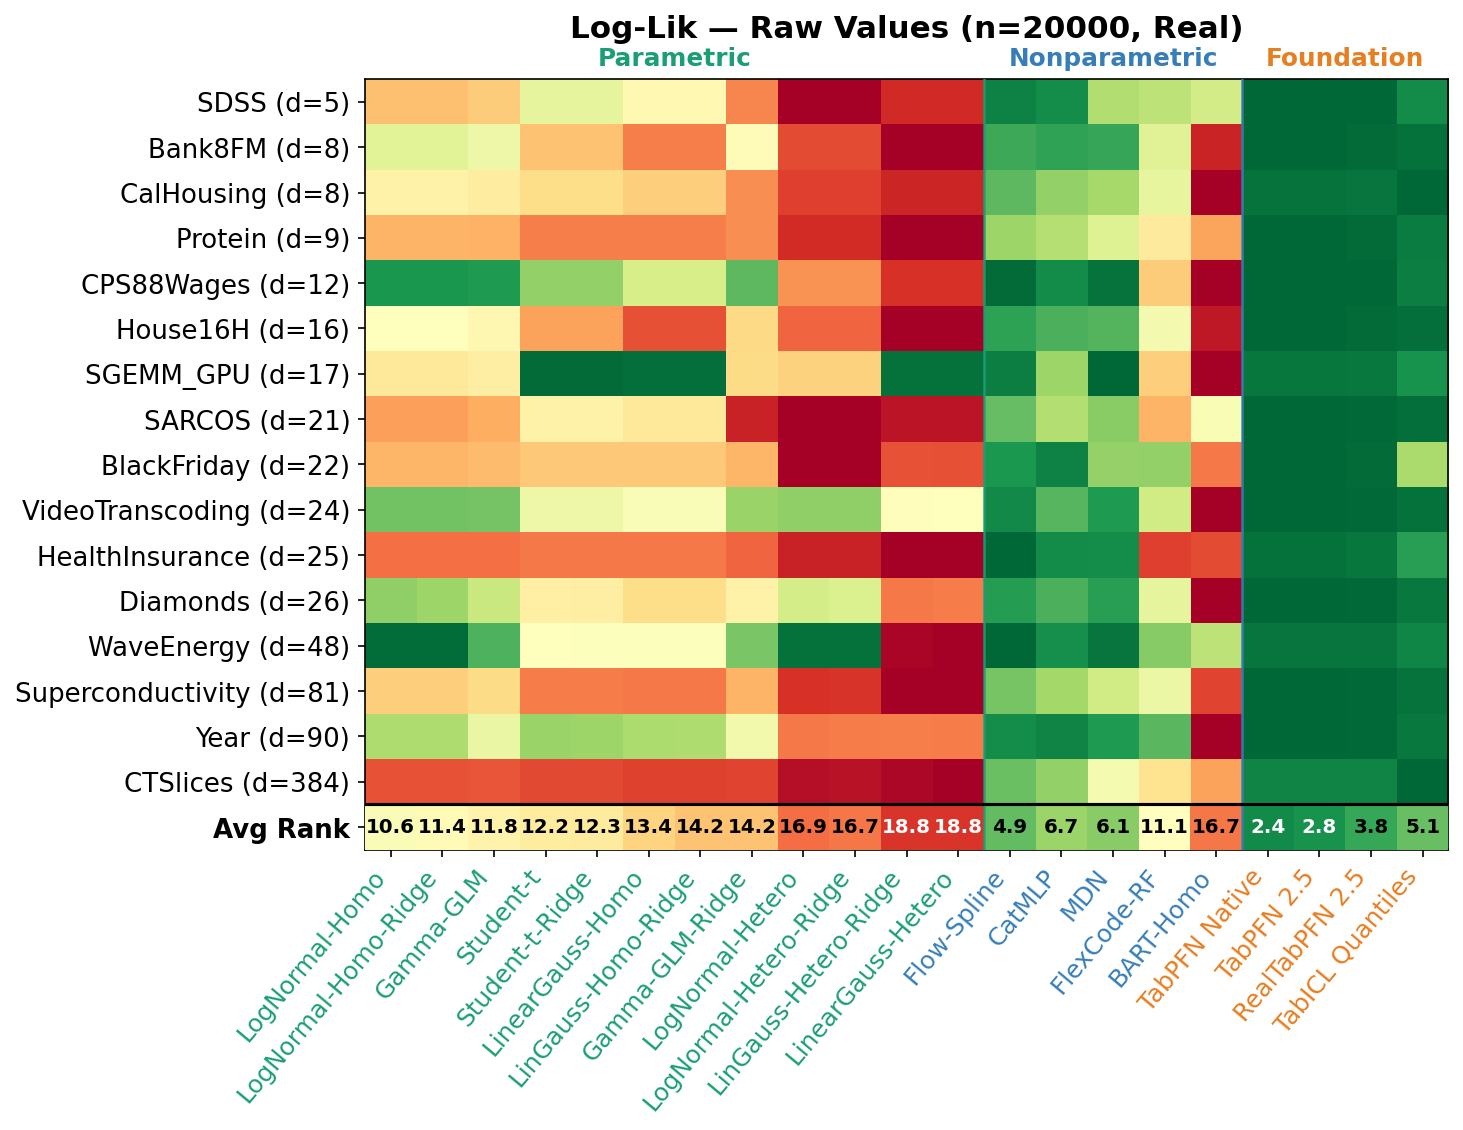
\includegraphics[width=\linewidth]{results_real/raw_real_log_lik_n20000.png}
  \caption{Raw Log-Likelihood -- $n=20000$, real data.}
\end{figure}

% ── CRPS ────────────────────────────────────────────────────────────────────
\subsubsection{CRPS}

\begin{figure}[p]\centering
  
\includegraphics[width=\linewidth]{results_real/raw_real_crps_n50.png}
  \caption{Raw CRPS -- $n=50$, real data.}
\end{figure}
\begin{figure}[p]\centering
  
\includegraphics[width=\linewidth]{results_real/raw_real_crps_n500.png}
  \caption{Raw CRPS -- $n=500$, real data.}
\end{figure}
\begin{figure}[p]\centering
  
\includegraphics[width=\linewidth]{results_real/raw_real_crps_n1000.png}
  \caption{Raw CRPS -- $n=1000$, real data.}
\end{figure}
\begin{figure}[p]\centering
  
\includegraphics[width=\linewidth]{results_real/raw_real_crps_n5000.png}
  \caption{Raw CRPS -- $n=5000$, real data.}
\end{figure}
\begin{figure}[p]\centering
  
\includegraphics[width=\linewidth]{results_real/raw_real_crps_n10000.png}
  \caption{Raw CRPS -- $n=10000$, real data.}
\end{figure}
\begin{figure}[p]\centering
  
\includegraphics[width=\linewidth]{results_real/raw_real_crps_n20000.png}
  \caption{Raw CRPS -- $n=20000$, real data.}
\end{figure}

% ── PIT KS ──────────────────────────────────────────────────────────────────
\subsubsection{PIT KS Statistic}

\begin{figure}[p]\centering
  
\includegraphics[width=\linewidth]{results_real/raw_real_pit_ks_n50.png}
  \caption{Raw PIT KS -- $n=50$, real data.}
\end{figure}
\begin{figure}[p]\centering
  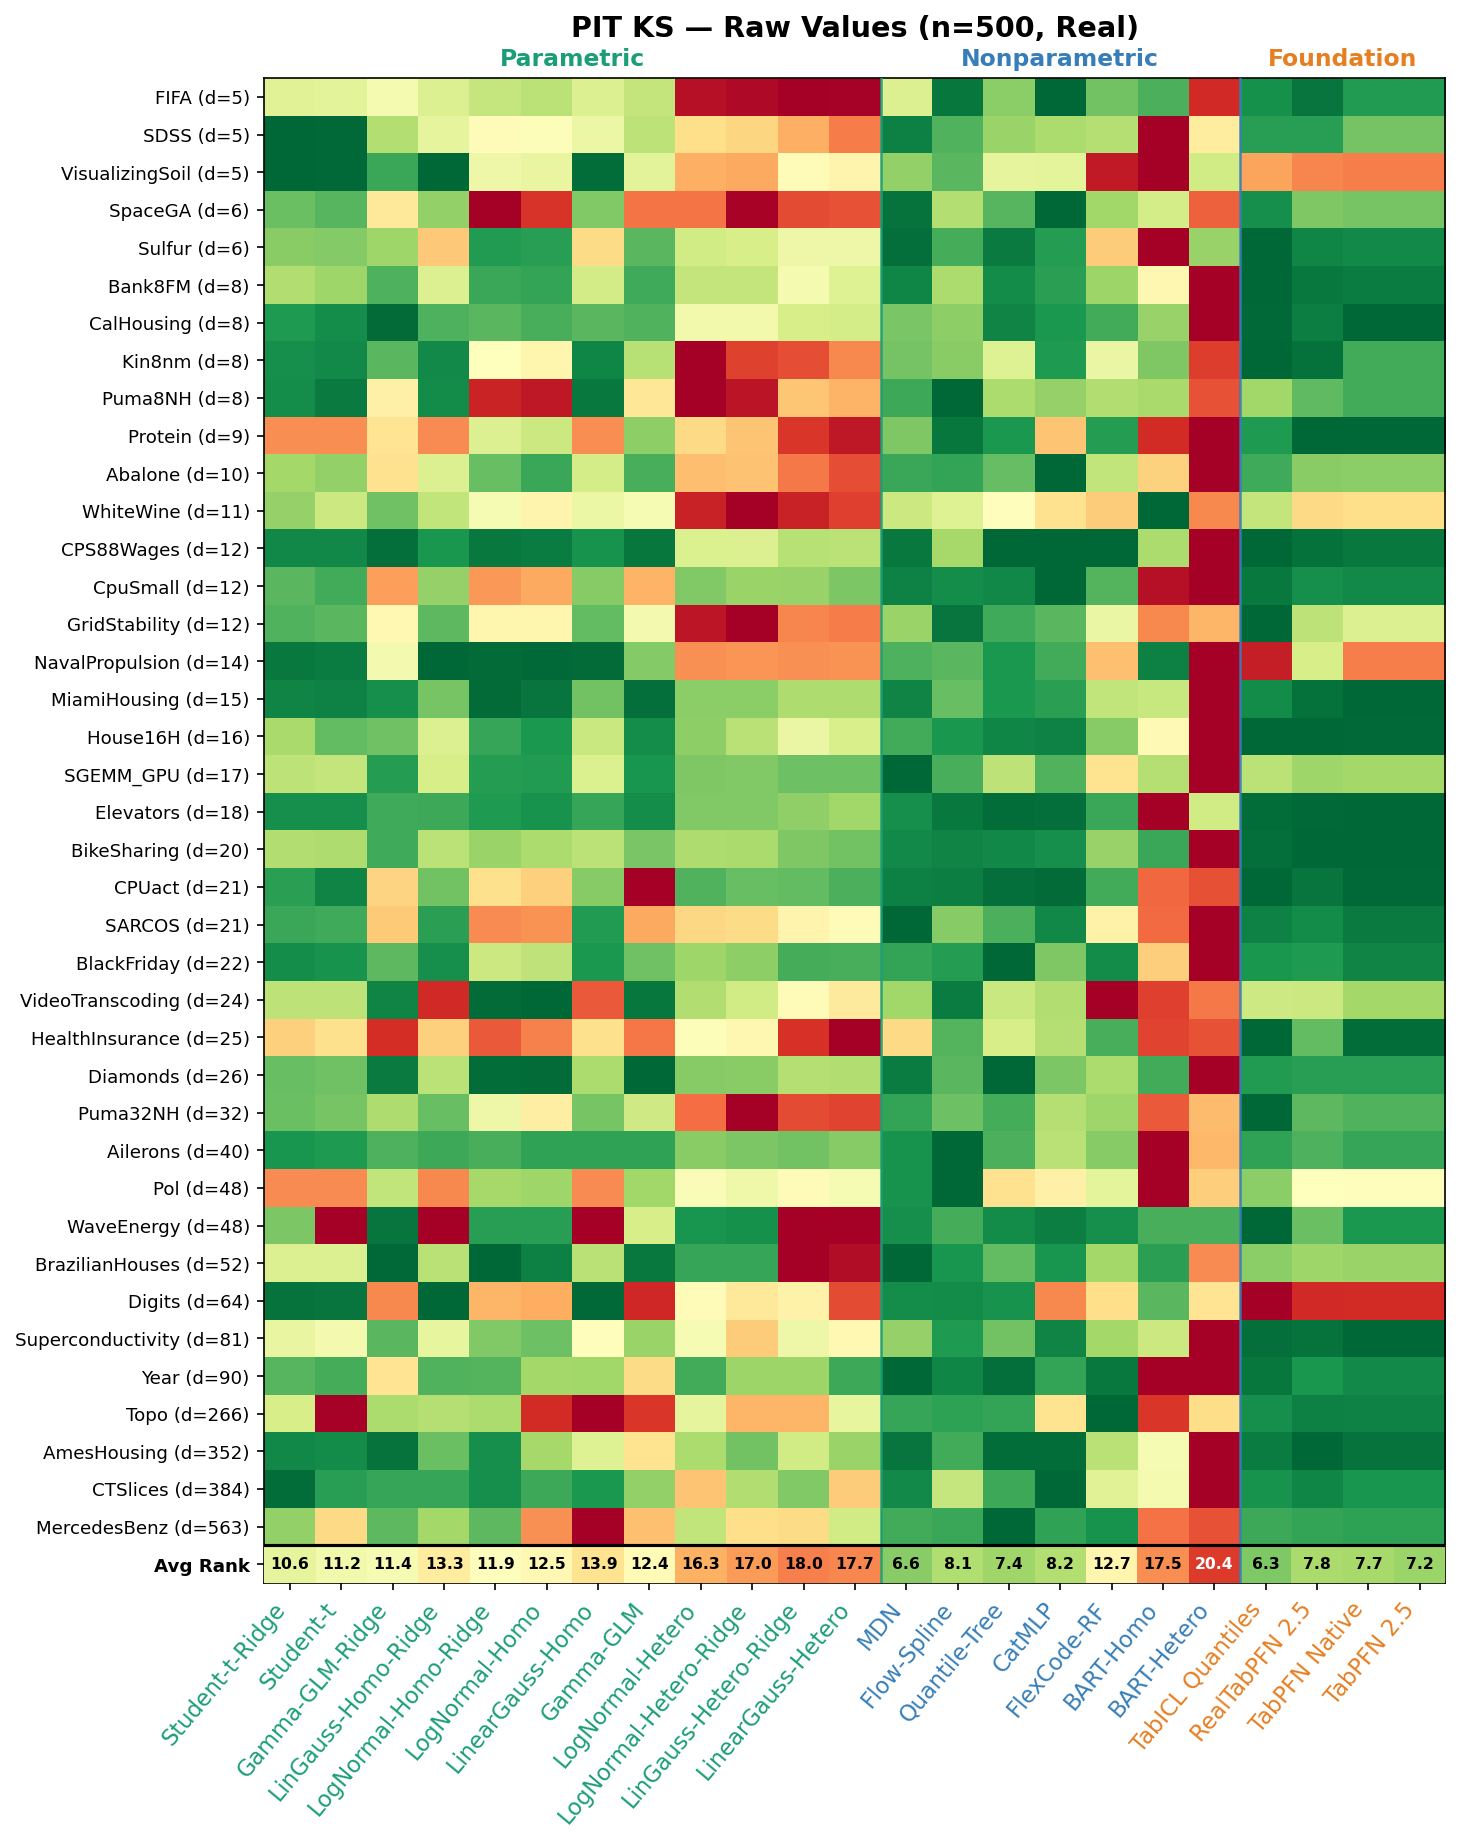
\includegraphics[width=\linewidth]{results_real/raw_real_pit_ks_n500.png}
  \caption{Raw PIT KS -- $n=500$, real data.}
\end{figure}
\begin{figure}[p]\centering
  
\includegraphics[width=\linewidth]{results_real/raw_real_pit_ks_n1000.png}
  \caption{Raw PIT KS -- $n=1000$, real data.}
\end{figure}
\begin{figure}[p]\centering
  
\includegraphics[width=\linewidth]{results_real/raw_real_pit_ks_n5000.png}
  \caption{Raw PIT KS -- $n=5000$, real data.}
\end{figure}
\begin{figure}[p]\centering
  
\includegraphics[width=\linewidth]{results_real/raw_real_pit_ks_n10000.png}
  \caption{Raw PIT KS -- $n=10000$, real data.}
\end{figure}
\begin{figure}[p]\centering
  
\includegraphics[width=\linewidth]{results_real/raw_real_pit_ks_n20000.png}
  \caption{Raw PIT KS -- $n=20000$, real data.}
\end{figure}

% ── 90\% Coverage ───────────────────────────────────────────────────────────
\subsubsection{90\% Coverage}

\begin{figure}[p]\centering
  
\includegraphics[width=\linewidth]{results_real/raw_real_coverage_90_n50.png}
  \caption{Raw 90\% Coverage -- $n=50$, real data.}
\end{figure}
\begin{figure}[p]\centering
  
\includegraphics[width=\linewidth]{results_real/raw_real_coverage_90_n500.png}
  \caption{Raw 90\% Coverage -- $n=500$, real data.}
\end{figure}
\begin{figure}[p]\centering
  
\includegraphics[width=\linewidth]{results_real/raw_real_coverage_90_n1000.png}
  \caption{Raw 90\% Coverage -- $n=1000$, real data.}
\end{figure}
\begin{figure}[p]\centering
  
\includegraphics[width=\linewidth]{results_real/raw_real_coverage_90_n5000.png}
  \caption{Raw 90\% Coverage -- $n=5000$, real data.}
\end{figure}
\begin{figure}[p]\centering
  
\includegraphics[width=\linewidth]{results_real/raw_real_coverage_90_n10000.png}
  \caption{Raw 90\% Coverage -- $n=10000$, real data.}
\end{figure}
\begin{figure}[p]\centering
  
\includegraphics[width=\linewidth]{results_real/raw_real_coverage_90_n20000.png}
  \caption{Raw 90\% Coverage -- $n=20000$, real data.}
\end{figure}

% ── Interval Width ──────────────────────────────────────────────────────────

% ── Fit Time ────────────────────────────────────────────────────────────────
\subsubsection{Fit Time}

\begin{figure}[p]\centering
  
\includegraphics[width=\linewidth]{results_real/raw_real_fit_time_n50.png}
  \caption{Raw Fit Time -- $n=50$, real data.}
\end{figure}
\begin{figure}[p]\centering
  
\includegraphics[width=\linewidth]{results_real/raw_real_fit_time_n500.png}
  \caption{Raw Fit Time -- $n=500$, real data.}
\end{figure}
\begin{figure}[p]\centering
  
\includegraphics[width=\linewidth]{results_real/raw_real_fit_time_n1000.png}
  \caption{Raw Fit Time -- $n=1000$, real data.}
\end{figure}
\begin{figure}[p]\centering
  
\includegraphics[width=\linewidth]{results_real/raw_real_fit_time_n5000.png}
  \caption{Raw Fit Time -- $n=5000$, real data.}
\end{figure}
\begin{figure}[p]\centering
  
\includegraphics[width=\linewidth]{results_real/raw_real_fit_time_n10000.png}
  \caption{Raw Fit Time -- $n=10000$, real data.}
\end{figure}
\begin{figure}[p]\centering
  
\includegraphics[width=\linewidth]{results_real/raw_real_fit_time_n20000.png}
  \caption{Raw Fit Time -- $n=20000$, real data.}
\end{figure}


\subsection{SDSS}



\end{document}
